% \documentclass[10pt]{beamer}
  \documentclass[9pt]{beamer}
% \usetheme{Madrid}
% \usetheme{Boadilla}
  \usetheme{default}
% \usetheme[numbering=counter]{metropolis}
  \definecolor{lightgray}{gray}{0.9}
% \definecolor{test1}{RGB}{250, 250, 230}
  \definecolor{test1}{RGB}{255, 255, 235}
  \definecolor{test2}{RGB}{240, 240, 250}
% \setbeamercolor{frametitle}{fg=black,bg=white}
  \setbeamercolor{frametitle}{fg=black,bg=test1}
  \setbeamercolor{background canvas}{bg=test2}
  \setbeamertemplate{frame footer}{UMBC Atmospheric Spectroscopy Lab}

\input{crisdefs.tex}

\title{A Quick Comparison of the UMBC, NOAA, and UW \\CrIS
       Calibration Algorithms}
\author{H.~E.~Motteler, L.~L.~Strow}

\institute{
  UMBC Atmospheric Spectroscopy Lab \\
  Joint Center for Earth Systems Technology \\
}
\date{12 Feb 2024}
\begin{document}

%----------- slide --------------------------------------------------%
\begin{frame}[plain]
\titlepage
\end{frame}
%----------- slide --------------------------------------------------%
\begin{frame}
\frametitle{Introduction}
\begin{itemize}

  \item We make several three-way comparisons of the UMBC, NOAA, and
    UW/NASA CrIS (Cross-track Infrared Sounder) calibrated radiance
    products, primarily for the J1/NOAA-20 sounder.

  \item These results are only spot checks of a few granules and
    FOVs, intended to look for obvious differences or problems.
    They were chosen as being representative of a larger number of
    tests.

  \item Overall, the three products look similar, at least for
    apodized radiances.  This is reassuring.  Different algorithms,
    and the presence or absence of a polarization correction, show
    up as measurable differences.

  \item Before showing differences, we take a quick look at
    reference truth and the polarization correction, the main
    causes of the differences.

\end{itemize}
\end{frame}
%----------- slide --------------------------------------------------%
\begin{frame}
\frametitle{Methods}
\begin{itemize}

  \item UMBC radiances are from UMBC CCAST versions V20 or V21,
    c. 2023, using the ``c7'' algorithm, except as noted.

  \item UW/NASA radiances are from their L1b V2 product, except as
    noted. 

  \item NOAA radiances are from the NOAA CrIS SDR production system,
    as of late 2023 and early 2024.

  \item the CCAST c7 algorithm uses a ``ratio-first'' calibration
    algorithm, periodic sinc at the decimated sensor grid for the
    ILS, cosine apodization at the band edges of the sensor grid,
    resampling to take the sensor to the user grid, and a sinc basis
    for reference truth.

  \item NOAA and UW use an ``SA-first'' algorithm, a sinc basis for
    the ILS, with an extended SA matrix, circular shift of the
    extended user grid, resampling, and reference truth convolved
    with instrument responsivity.  NOAA and UW V3 include a
    polarization correction, while UMBC and UW V2 do not.

  \item Fundamental calibration equations are given in the appendix.

\end{itemize}
\end{frame}
%----------- slide --------------------------------------------------%
\begin{frame}
\frametitle{Reference truth}
\begin{itemize}

  \item Reference truth is calculated upwelling radiance---what we
    expect the sounder to see for a particular atmospheric state.

  \item We generate this starting with kcarta, which gives an
    approximation to line-by-line calculations at an $0.0025 \wn$
    grid, and convolve the result to match instrument OPD,
    passbands, and filter specs.

  \item This is a conventional method for calculating reference
    truth.  However NOAA and UW/NASA do something different---they
    convolve reference truth as above with instrument responsivity,
    and use this modified reference truth for instrument validation.

  \item There are problems with this.  Mainly, it amounts to trying
    to define away an error, rather than fixing it.  In addition,
    responsivity varies among the CrIS family of sounders, so that
    you have no single, even nominal, reference truth.

  \item As the following plot shows, the difference is significant
    for unapodized radiances, more than 0.2 K at many points.

%  More than anything else, a flame is expository writing.
%  -- Curtis Yarvin.

\end{itemize}
\end{frame}
%----------- slide --------------------------------------------------%
\begin{frame}
\frametitle{Responsivity vs flat reference truth}
\begin{center}
  
\includegraphics[scale=0.45]{figures/resp_flat_diff.pdf}
\end{center}
\end{frame}
%----------- slide --------------------------------------------------%
\begin{frame}
\frametitle{Validation}
\begin{itemize}

  \item The UMBC calibration algorithm was validated with simple
    ``flat'' reference truth, with a sinc basis, while NOAA and
    UW/NASA were validated with reference truth convolved with
    instrument responsivity.

  \item What this means in practice is that even if everything else
    was perfect, their respective calibrated radiance products would
    differ by the difference of responsivity vs flat reference
    truth, as shown above.

  \item This is a significant part of what we see in the unapodized
    differences that we show below.

  \item Note that most of the differences disappear with moderate
    apodization, as is often applied in practice.  But there are
    cases where we would like to use the full resolution of the
    instrument.

  \item A list of UMBC validation presentations is given in the
    appendix.  These (and in particular ccast\_noaa3 and 4) show UMBC
    and NOAA are in good agreement with their respective values for
    reference truth.  The reports are bundled with the ccast git
    repo.

\end{itemize}
\end{frame}
%----------- slide --------------------------------------------------%
\begin{frame}
\frametitle{Polarization correction}
\begin{itemize}

  \item We see the effect of different reference truth mostly at
    higher spectral resolutions (that is, at a finer frequency
    grid).  These differences largely disappear with apodization.

  \item In contrast, the polarization correction gives rise to
    significant differences at lower spectral resolutions (a coarser
    grid) which persist with apodization.

  \item NOAA and UW V3 include a polarization correction, while UMBC
    and UW V2 do not.

  \item In the following slide, we show the polarization correction
    as the difference of UW v2 and v3 over all obs for 5 Oct 2023,
    for Hamming apodized radiances.  Stats are done with brightness
    temps.  std is the std of the differences, not the difference of
    separate v2 and v3 stds.  In addition to the polarization
    correction, we see v3 has a significant cold bias, relative to
    v2.

\end{itemize}
\end{frame}
%----------- slide --------------------------------------------------%
\begin{frame}
\frametitle{Polarization correction}
\begin{center}
  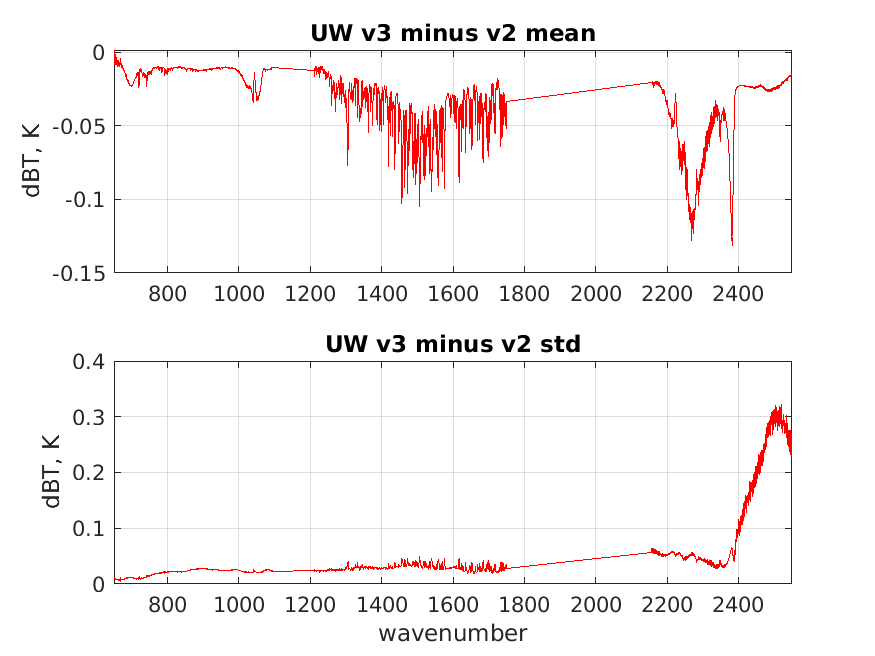
\includegraphics[scale=0.25]{figures/UW_v3_minus_v2.png}
\end{center}

UW v3 minus v2 for 5 Oct 2023, for Hamming apodized radiances.
Stats are done with brightness temp.  std is the std of the
differences, not the difference of separate v2 and v3 stds.  In
addition to the polarization correction, we see v3 has a significant
cold bias, relative to v2.

\end{frame}
%----------- slide --------------------------------------------------%
\begin{frame}
\frametitle{LW unapodiazed comparisons} % (Oct 14)

\begin{columns}[t]

\begin{column}{0.5\textwidth}
  \begin{centering}
  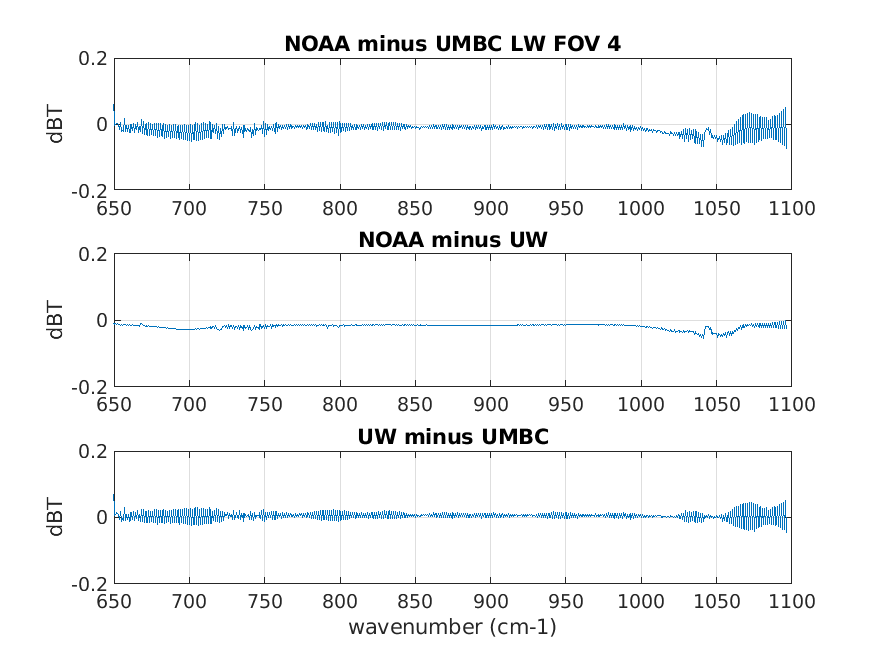
\includegraphics[width=\textwidth]{figures/LW_FOV4_unap_SDR_diffs.png}
  \end{centering}\vspace{3mm}
\end{column}

\begin{column}{0.5\textwidth}
  \begin{centering}
  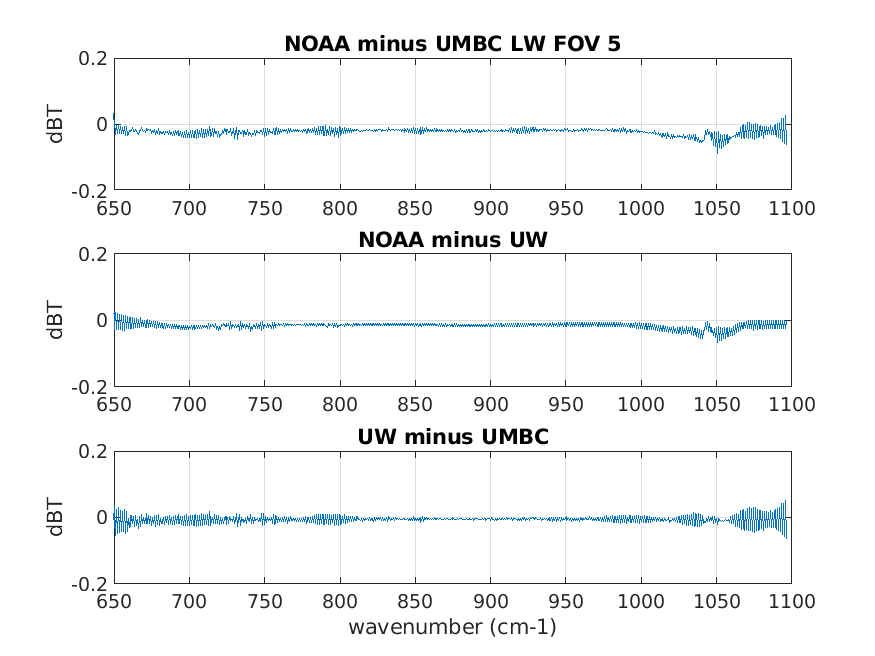
\includegraphics[width=\textwidth]{figures/LW_FOV5_unap_SDR_diffs.png}
  \end{centering}\vspace{3mm}
\end{column}

\end{columns}
 
A 3-way comparison of NOAA, UMBC, and UW, LW unapodized radiances,
for FOVs 4 and 5.  Results are for J1/NOAA-20, 5 Oct 2023, UTC 19:03,
lat 55 lon -97, 1200 matching obs, all FORs.

\end{frame}
%----------- slide --------------------------------------------------%
\begin{frame}
\frametitle{MW unapodiazed comparisons} % (Oct 14)

\begin{columns}[t]

\begin{column}{0.5\textwidth}  
  \begin{centering}
  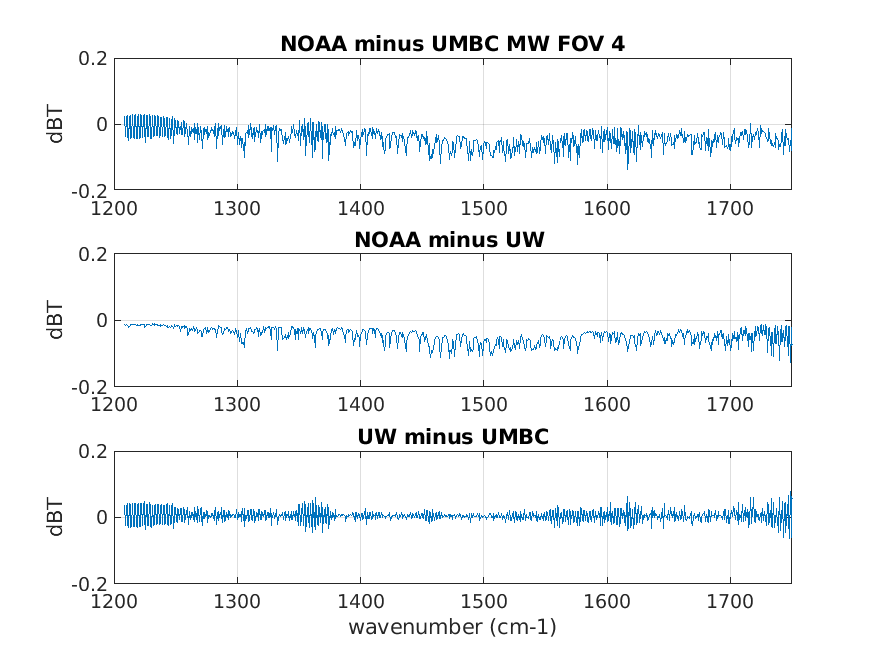
\includegraphics[width=\textwidth]{figures/MW_FOV4_unap_SDR_diffs.png}
  \end{centering}\vspace{3mm}
\end{column}

\begin{column}{0.5\textwidth}  
  \begin{centering}
  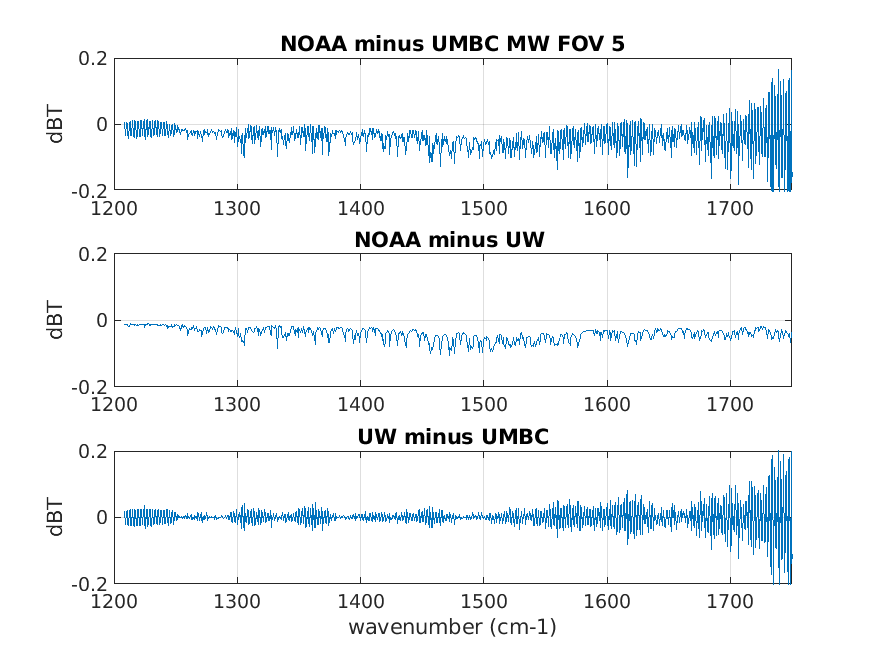
\includegraphics[width=\textwidth]{figures/MW_FOV5_unap_SDR_diffs.png}
  \end{centering}\vspace{3mm}
\end{column}

\end{columns}

A 3-way comparison of NOAA, UMBC, and UW, MW unapodized radiances,
for FOVs 4 and 5.  Results are for J1/NOAA-20, 5 Oct 2023, UTC 19:03,
lat 55 lon -97, 1200 matching obs, all FORs.

\end{frame}
%----------- slide --------------------------------------------------%
\begin{frame}
\frametitle{SW unapodized comparisons} % (Oct 14)

\begin{columns}[t]
 
\begin{column}{0.5\textwidth}  
  \begin{centering}
  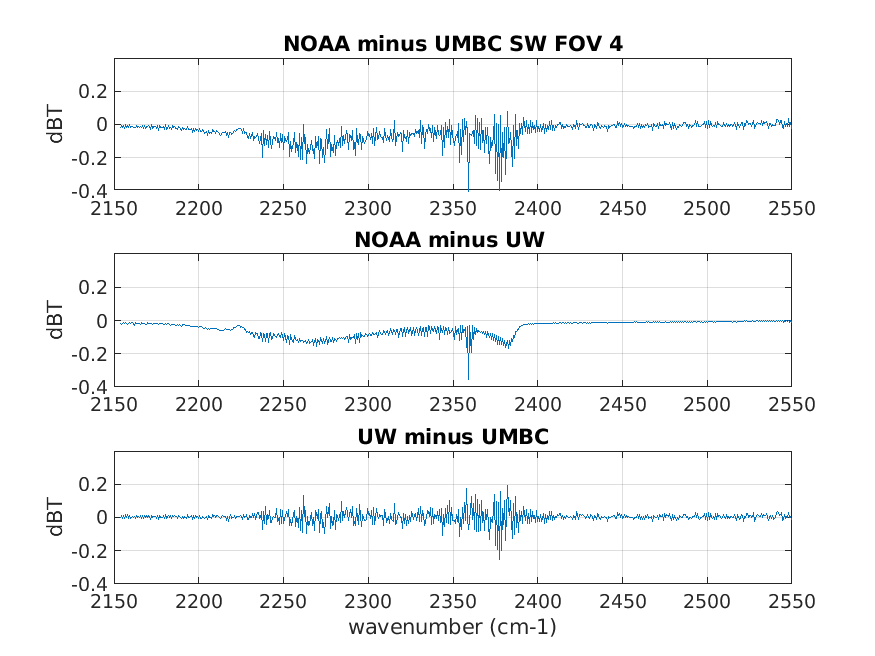
\includegraphics[width=\textwidth]{figures/SW_FOV4_unap_SDR_diffs.png}
  \end{centering}\vspace{3mm}
\end{column}

\begin{column}{0.5\textwidth}
  \begin{centering}
  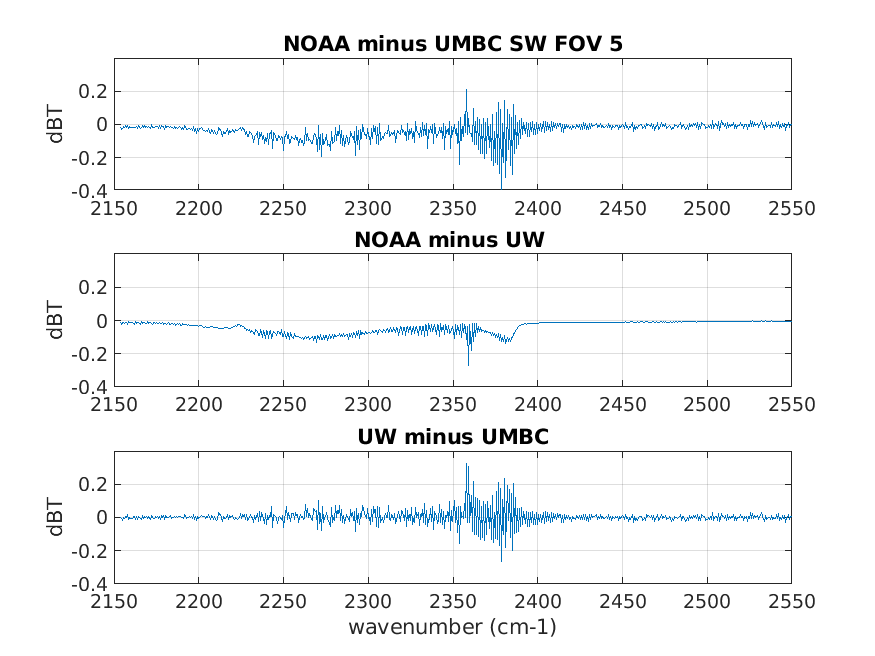
\includegraphics[width=\textwidth]{figures/SW_FOV5_unap_SDR_diffs.png}
  \end{centering}\vspace{3mm}
\end{column}

\end{columns}

A 3-way comparison of NOAA, UMBC, and UW, SW unapodized radiances,
for FOVs 4 and 5.  Results are for J1/NOAA-20, 5 Oct 2023, UTC
19:03, lat 55 lon -97, 1200 matching obs, all FORs.  Note the range
of the Y axis has been extended to $\pm 0.4$.

\end{frame}
%----------- slide --------------------------------------------------%
\begin{frame}
\frametitle{LW \& MW apodized comparisons} % (Jan 31)

\begin{columns}[t]
\begin{column}{0.5\textwidth}  
  \begin{centering}
  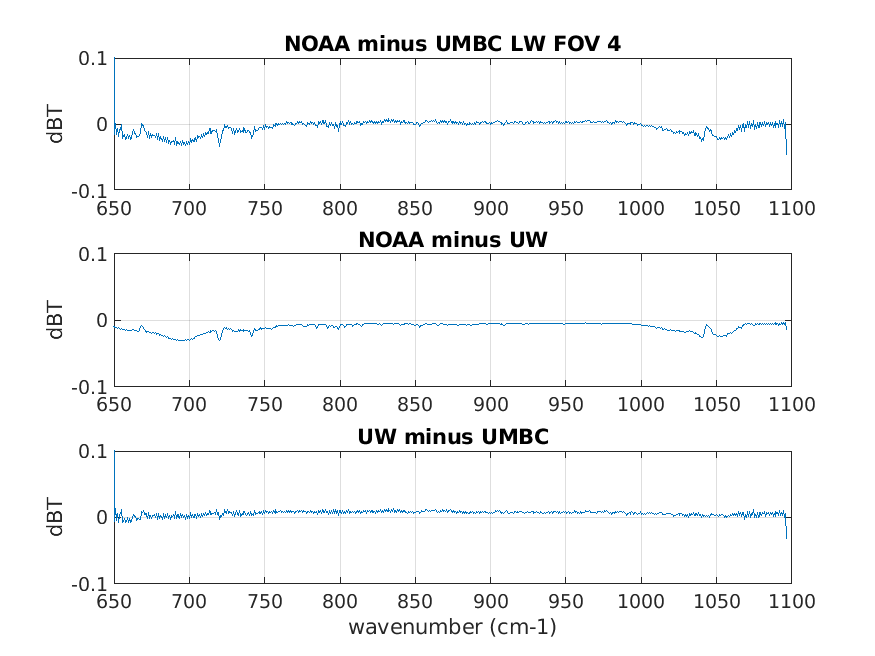
\includegraphics[width=\textwidth]{figures/LW_FOV4_hamm_SDR_diffs.png}
  \end{centering}\vspace{3mm}
 
\end{column}
 
\begin{column}{0.5\textwidth}
  \begin{centering}
  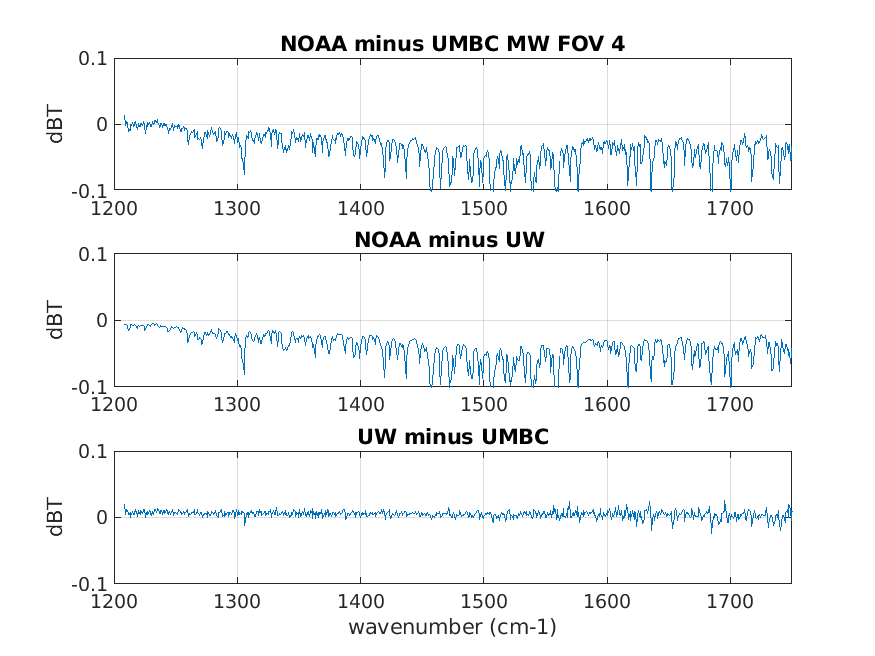
\includegraphics[width=\textwidth]{figures/MW_FOV4_hamm_SDR_diffs.png}
  \end{centering}\vspace{3mm}
 
\end{column}
\end{columns}

A 3-way comparison of NOAA, UMBC, and UW, LW and MW Hamming apodized
radiances, for FOV 4.  Results are for J1/NOAA-20, 05-Oct-2023
UTC 07:03:14, lat 21.9 lon 91.8, with 1170 matching obs, all FORs.
Note the range of the Y axis has been reduced to $\pm 0.1$.

\end{frame}
%----------- slide --------------------------------------------------%
\begin{frame}
\frametitle{SW apodized comparisons} % (Jan 31)

\begin{columns}[t]
\begin{column}{0.5\textwidth}  
  \begin{centering}
  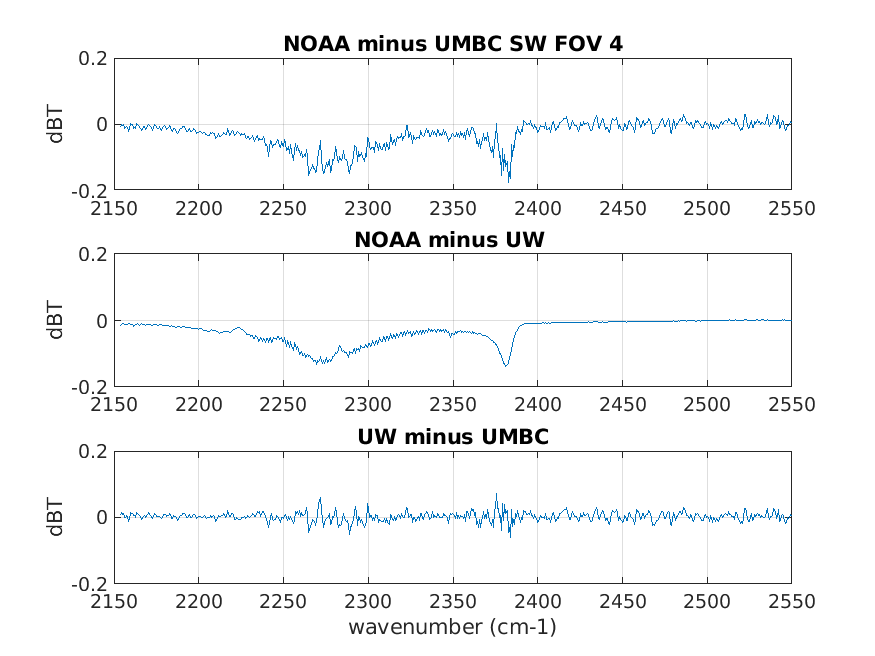
\includegraphics[width=\textwidth]{figures/SW_FOV4_hamm_SDR_diffs.png}
  \end{centering}\vspace{3mm}
 
\end{column}
 
\begin{column}{0.5\textwidth}
  \begin{centering}
% 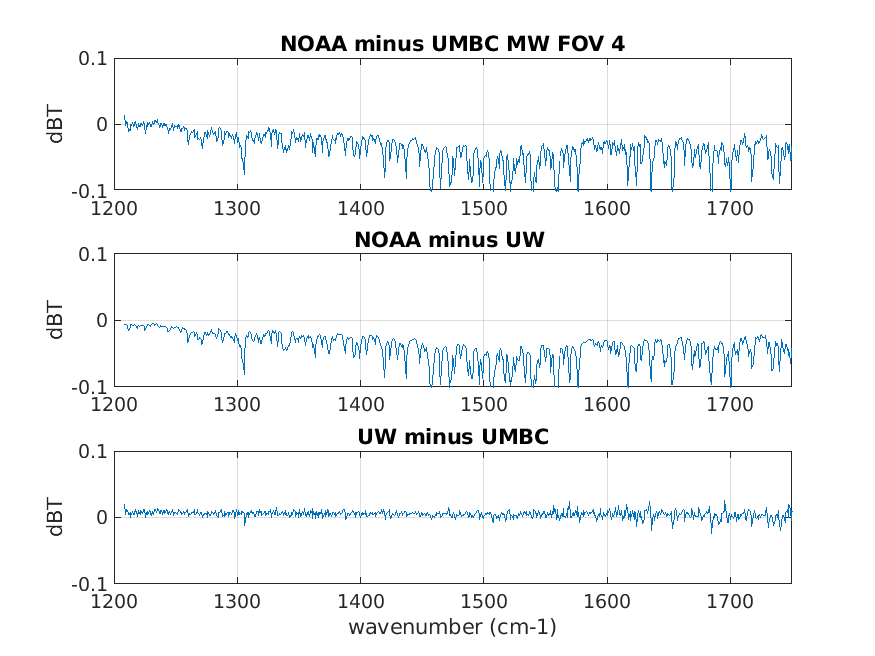
\includegraphics[width=\textwidth]{figures/MW_FOV4_hamm_SDR_diffs.png}
  \end{centering}\vspace{3mm}
 
\end{column}
\end{columns}

A 3-way comparison of NOAA, UMBC, and UW, SW Hamming apodized
radiances, for FOV 4.  Results are for J1/NOAA-20, 05-Oct-2023
UTC 07:03:14, lat 21.9 lon 91.8, with 1170 matching obs, all FORs.
Note the range of the Y axis is $\pm 0.2$K for this plot.

\end{frame}
%----------- slide --------------------------------------------------%
\begin{frame}
\frametitle{Discussion I}
\begin{itemize}

  \item The apodized differences between UW and UMBC are very
    small, for all three bands.  Given the significant differences in
    the processing algorithms, this is reassuring.

  \item The unapodized differences between UW and UMBC appear to be
    mainly due to the different calibration algorithms and reference
    truth.

  \item The apodized differences between NOAA and UMBC, and NOAA and
    UW, appear to be due mainly to the polarization correction.

  \item The unapodized differences between NOAA and UMBC appear to
    be a mix of differences due to the calibration algorithms and
    polarization correction.

  \item The unapodized differences between NOAA and UW appear to be
    due to the polarization correction. \bigskip\medskip

  \item In the following slides we compare NOAA and UW with the UMBC
    ``a4'' algorithm.

\end{itemize}
\end{frame}
%----------- slide --------------------------------------------------%
\begin{frame}
\frametitle{Unapodized a4 comparisons} % (2 Feb)

\begin{columns}[t]
\begin{column}{0.5\textwidth}  
  \begin{centering}
  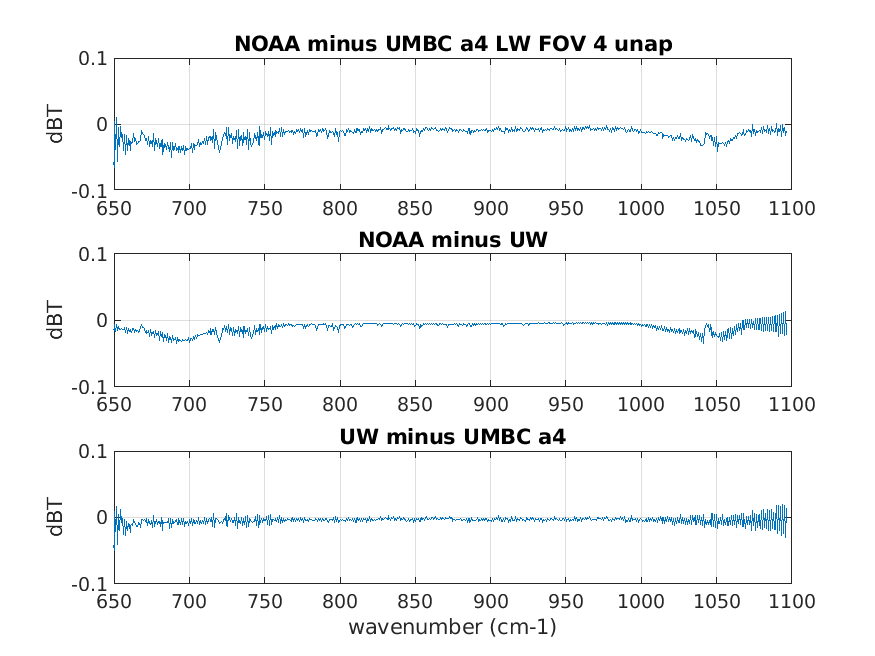
\includegraphics[width=\textwidth]{figures/LW_FOV4_a4_unap_SDR_diffs.png}
  \end{centering}\vspace{3mm}
 
\end{column}
 
\begin{column}{0.5\textwidth}
  \begin{centering}
  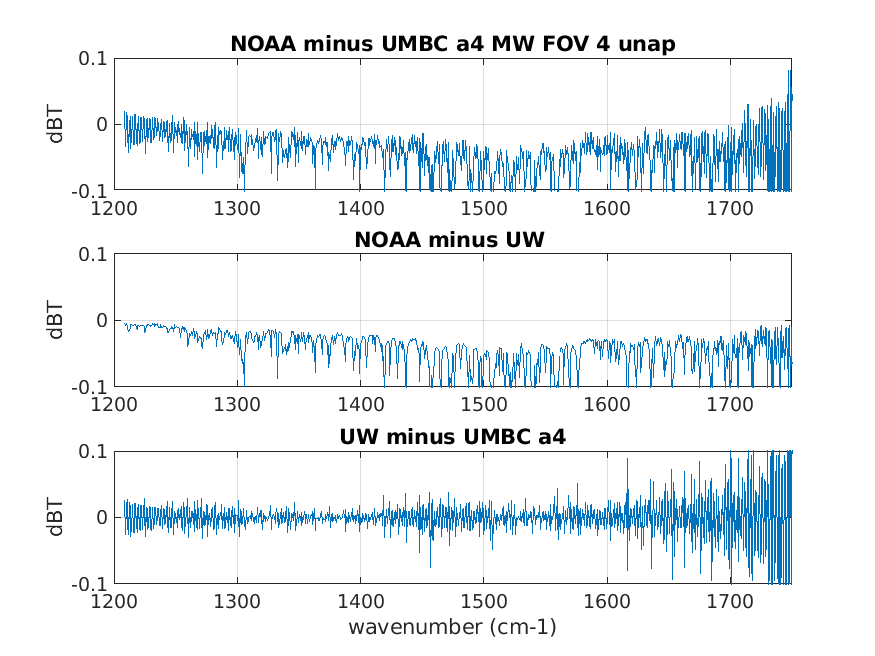
\includegraphics[width=\textwidth]{figures/MW_FOV4_a4_unap_SDR_diffs.png}
  \end{centering}\vspace{3mm}

  
\end{column}
\end{columns}

3-way comparison of NOAA, UMBC A4, and UW, LW and MW unapodized
radiances, for FOV 4.  Results are for J1/NOAA-20, 05-Oct-2023 UTC
07:03:14, lat 21.9 lon 91.8, with 1170 matching obs, all FORs.  Note
the range of the Y axis is $\pm 0.1$K for these plots.

\end{frame}
%----------- slide --------------------------------------------------%
\begin{frame}
\frametitle{Unapodized a4 comparisons} % (2 Feb)

\begin{columns}[t]
\begin{column}{0.5\textwidth}  
  \begin{centering}
  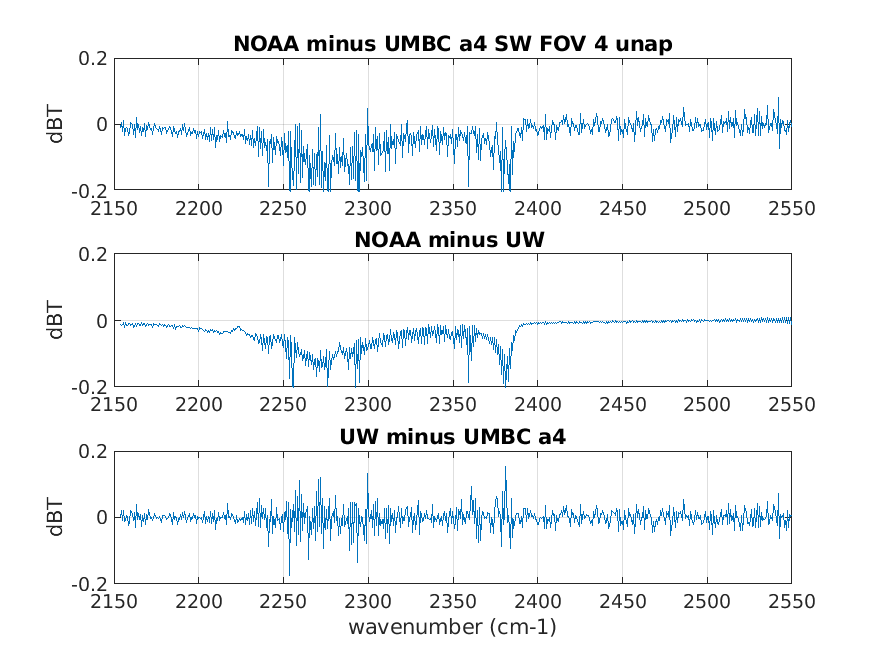
\includegraphics[width=\textwidth]{figures/SW_FOV4_a4_unap_SDR_diffs.png}
  \end{centering}\vspace{3mm}
 
\end{column}
 
\begin{column}{0.5\textwidth}
  \begin{centering}
% \includegraphics[width=\textwidth]{figures/}
  \end{centering}\vspace{3mm}
 
\end{column}
\end{columns}

3-way comparison of NOAA, UMBC A4, and UW SW Hamming apodized
radiances, for FOV 4.  Results are for J1/NOAA-20, 05-Oct-2023 UTC
07:03:14, lat 21.9 lon 91.8, with 1170 matching obs, all FORs.  Note
the range of the Y axis is $\pm 0.2$K for these plots.

\end{frame}
%----------- slide --------------------------------------------------%
\begin{frame}
\frametitle{Apodized a4 comparisons} % (2 Feb)

\begin{columns}[t]
\begin{column}{0.5\textwidth}  
  \begin{centering}
  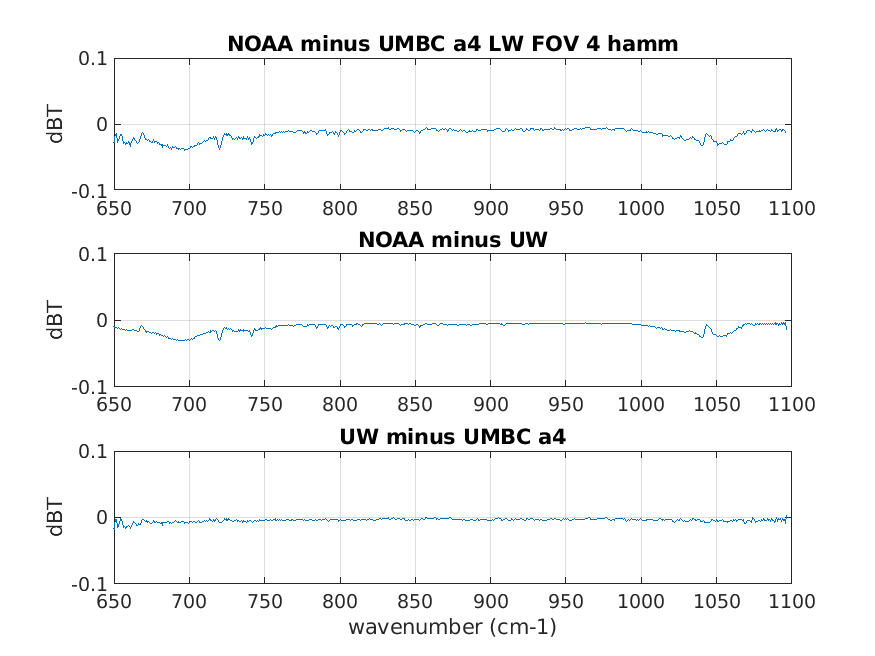
\includegraphics[width=\textwidth]{figures/LW_FOV4_a4_hamm_SDR_diffs.png}
  \end{centering}\vspace{3mm}
 
\end{column}
 
\begin{column}{0.5\textwidth}
  \begin{centering}
  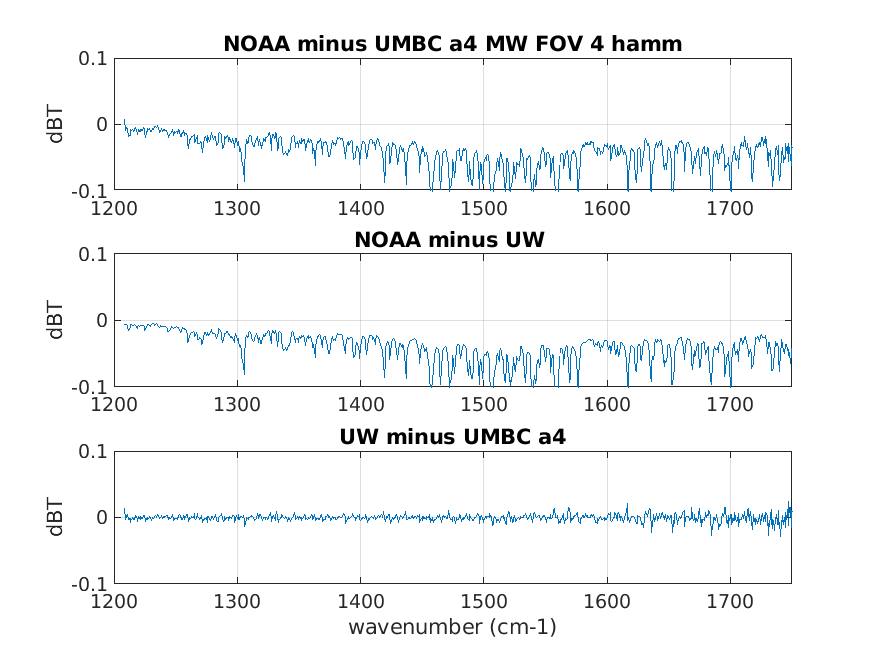
\includegraphics[width=\textwidth]{figures/MW_FOV4_a4_hamm_SDR_diffs.png}
  \end{centering}\vspace{3mm}
 
\end{column}
\end{columns}

3-way comparison of NOAA, UMBC A4, and UW, LW and MW, Hamming
apodized radiances, for FOV 4.  Results are for J1/NOAA-20,
05-Oct-2023 UTC 07:03:14, lat 21.9 lon 91.8, with 1170 matching obs,
all FORs.  Note the range of the Y axis is $\pm 0.1$K for these
plots.

\end{frame}
%----------- slide --------------------------------------------------%
\begin{frame}
\frametitle{Apodized a4 comparisons}
% (2 Feb)

\begin{columns}[t]
\begin{column}{0.5\textwidth}  
  \begin{centering}
  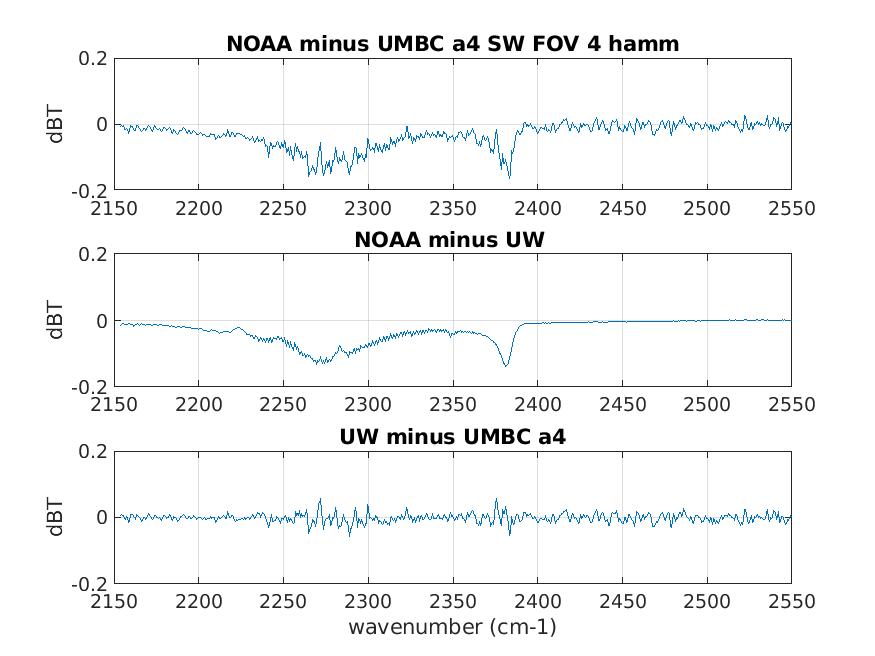
\includegraphics[width=\textwidth]{figures/SW_FOV4_a4_hamm_SDR_diffs.png}
  \end{centering}\vspace{3mm}
 
\end{column}
 
\begin{column}{0.5\textwidth}
  \begin{centering}
% 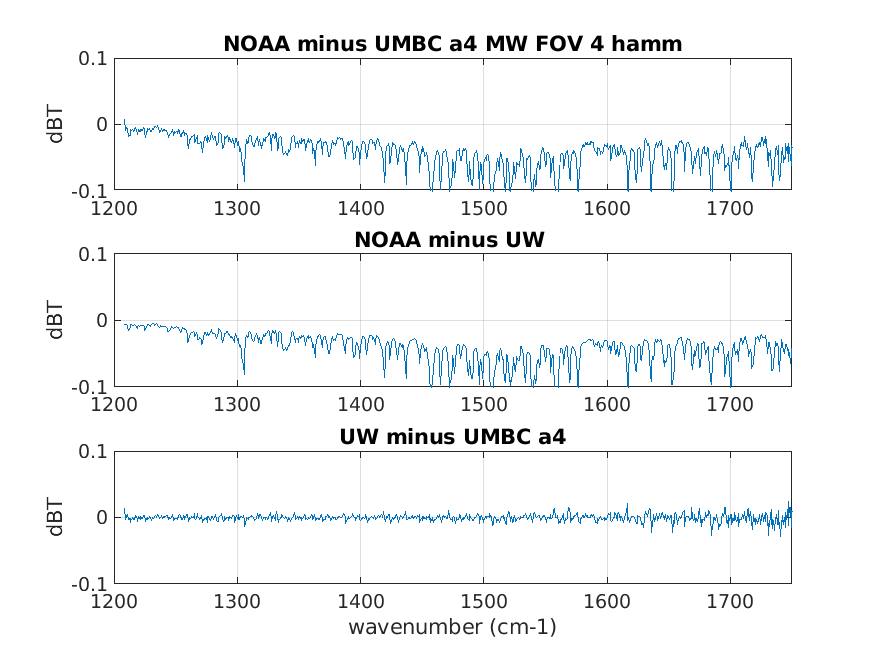
\includegraphics[width=\textwidth]{figures/MW_FOV4_a4_hamm_SDR_diffs.png}
  \end{centering}\vspace{3mm}
 
\end{column}
\end{columns}

3-way comparison of NOAA, UMBC A4, and UW, SW Hamming apodized
radiances, for FOV 4.  Results are for J1/NOAA-20, 05-Oct-2023 UTC
07:03:14, lat 21.9 lon 91.8, with 1170 matching obs, all FORs.  Note
the range of the Y axis is $\pm 0.2$K for these plots.

\end{frame}
%----------- slide --------------------------------------------------%
\begin{frame}
\frametitle{Unapodized c7 comparisons} % (2 Feb)

\begin{columns}[t]
\begin{column}{0.5\textwidth}  
  \begin{centering}
  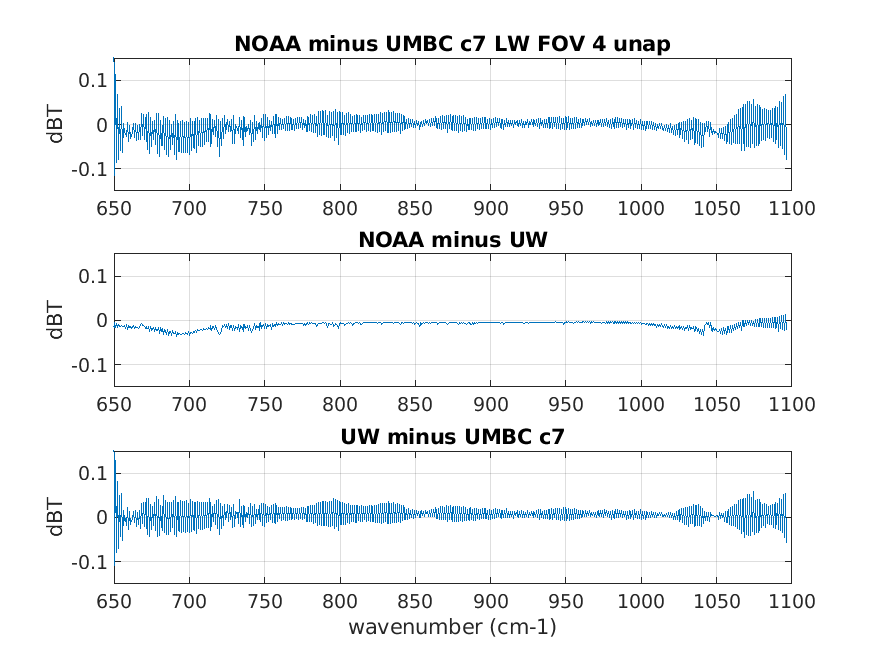
\includegraphics[width=\textwidth]{figures/LW_FOV4_c7_unap_SDR_diffs.png}
  \end{centering}\vspace{3mm}
 
\end{column}
 
\begin{column}{0.5\textwidth}
  \begin{centering}
  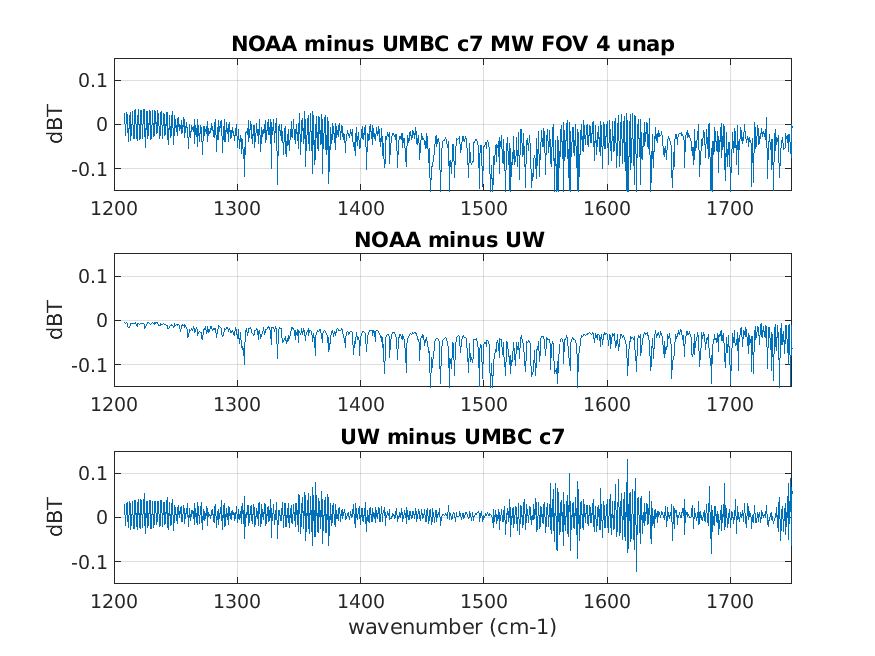
\includegraphics[width=\textwidth]{figures/MW_FOV4_c7_unap_SDR_diffs.png}
  \end{centering}\vspace{3mm}

  
\end{column}
\end{columns}

3-way comparison of NOAA, UMBC c7, and UW, LW and MW unapodized
radiances, for FOV 4.  Results are for J1/NOAA-20, 05-Oct-2023 UTC
07:03:14, lat 21.9 lon 91.8, with 1170 matching obs, all FORs.  Note
this is the same test method as the 5 Oct 2023 UTC 19:03 tests, but
with different data.  The range of the Y axis is $\pm 0.15$K for
these plots.

\end{frame}
%----------- slide --------------------------------------------------%
\begin{frame}
\frametitle{Unapodized c7 comparisons} % (2 Feb)

\begin{columns}[t]
\begin{column}{0.5\textwidth}  
  \begin{centering}
  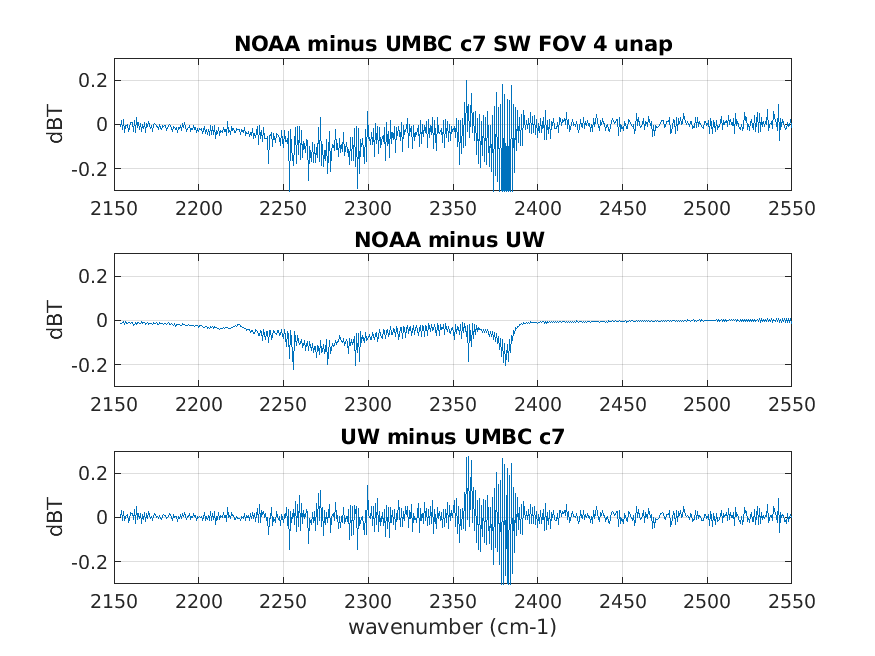
\includegraphics[width=\textwidth]{figures/SW_FOV4_c7_unap_SDR_diffs.png}
  \end{centering}\vspace{3mm}
 
\end{column}
 
\begin{column}{0.5\textwidth}
  \begin{centering}
% \includegraphics[width=\textwidth]{figures/}
  \end{centering}\vspace{3mm}
 
\end{column}
\end{columns}

3-way comparison of NOAA, UMBC c7, and UW, SW unapodized radiances,
for FOV 4.  Results are for J1/NOAA-20, 05-Oct-2023 UTC 07:03:14,
lat 21.9 lon 91.8, with 1170 matching obs, all FORs.  Note this is
the same test method as the 5 Oct 2023 UTC 19:03 tests, but with
different data.  The range of the Y axis is $\pm 0.3$K for this plot.

\end{frame}
%----------- slide --------------------------------------------------%
\begin{frame}
\frametitle{Discussion II}
\begin{itemize}

  \item UMBC A4 is the UMBC implementation of the ``SA first''
    algorithm used by NOAA and UW.  In general these residuals are
    smaller, as we would expect.  In this group of plots we are only
    showing FOV 4, for which the unapodized residuals were
    relatively large.

  \item The NOAA minus UMBC and UW minus UMBC unapodized residuals
    are similar in shape, but about half the size of the residuals
    from slides 9--11, where UMBC used the C7 algorithm.  Note
    that these are for the same day but different granules.

  \item The NOAA minus UW unapodized residuals are almost identical
    to the residuals from slides 9--11.  This is as we would
    expect, since the the only change is that we are looking at
    different granules.

  \item The NOAA minus UMBC and UW minus UMBC apodized residuals are
    almost identical to the residuals from slides 12 and 13.  Again
    this is to be expected, since the change is from UMBC C7 to A4,
    which has very little effect on apodized radiances.

  \item Finally, the unapodized c7 comparisons (slides 19--20) are
    very similar to the earlier unapodized c7 comparisons (slides
    9-11), since the only difference is the data.


\end{itemize}
\end{frame}
%----------- slide --------------------------------------------------%
\begin{frame}
\frametitle{Conclusions}
\begin{itemize}

  \item We did a 3-way comparison of CrIS calibrated radiance
    products, in the form of spot checks for a few granules and
    FOVs, primarily for the J1/NOAA-20 sounder.  Overall, the
    products look similar, at least for apodized radiances.

  \item Differences in unapodized radiances, up to a little more
    than 0.2 K, are mainly due to different calibration algorithms,
    validated with different versions of reference truth, and also
    in part due to the presence or absence of a polarization
    correction.

  \item Differences in apodized radiances, up to a little more than
    0.1 K, are mainly due to the presence or absence of a
    polarization correction.

  \item Other differences are due to different calibration
    algorithms and other processing details.  The validation
    reports, and in particular ccast\_noaa3, ccast\_noaa4, and
    cris\_psinc.pdf, in the ccast repo, have more detail.

\end{itemize}
\end{frame}
%----------- slide --------------------------------------------------%
\begin{frame}
\frametitle{Future work}
\begin{itemize}

  \item Unfortunately, UMBC CCAST lacks a polarization correction,
    and a few other desirable features such as a Doppler correction.
    Development mostly stopped after around 2020, aside from apps
    for TVAC and post-launch validation, and there are no resources
    or clear demand for further work.
  
  \item Even lacking the polarization correction, CCAST may still be
    superior when an unapodized product or fast processing is
    desired.  See the README in the CCAST git repo for a summary of
    the ways in which CCAST and the NOAA and UW products differ.

  \item We got much ``mileage'' out of CCAST over the years,
    processing and reprocessing the CrIS observations up to around
    2023.  We still use many of the libs and procedures for things
    like the J1-J4 TVAC analysis, focal plane fitting, validation
    after launch, and so on.

  \item We should have written a validation paper for CCAST.
    However the time for that was probably ten years ago.

  \item This presentation was reconstructed from Slack discussions
    from late 2023 and early 2024.

\end{itemize}
\end{frame}
%----------- slide --------------------------------------------------%
\begin{frame}
\frametitle{CCAST calibration equations}

% \begin{equation}
%   \rES = F \cdot \rIT \cdot f \cdot \SA^{-1}\cdot f \cdot 
%          \frac{\ES - \SPmean}{\ITmean - \SPmean}
% \end{equation}

\begin{center}
{\ccast} reference equation
\end{center}
\vspace{-2mm}
\begin{equation}
  \rESuser = F \cdot \rITsensor \cdot \fcos \cdot \SA^{-1}\cdot \fcos 
         \cdot \frac{\Delta\ES}{\Delta\IT}
\end{equation}

\begin{equation}
  \rESuser = F \cdot \fcos \cdot \SA^{-1}\cdot \fcos \cdot \rITfov 
         \cdot \frac{\Delta\ES}{\Delta\IT}
\end{equation}

\vspace{3mm}
\begin{center}
{\noaa} algorithm 4
\end{center}
\vspace{-2mm}
\begin{equation}
  \rESuser = \rITuser \cdot
         \frac{F \cdot \fatbd \cdot \SA^{-1}\cdot \fatbd \cdot 
                  (\frac{\Delta\ES}{\Delta\IT}) \cdot {|\Delta\IT|}}
              {F \cdot \fatbd \cdot \SA^{-1}\cdot \fatbd \cdot {|\Delta\IT|}}
\end{equation}

\vspace{3mm}
\[ \Delta\ES = \ES - \SPmean, \hspace{4mm}
   \Delta\IT = \ITmean - \SPmean \]

\end{frame}
%----------- slide --------------------------------------------------%
\begin{frame}
\frametitle{Calibration equation parameters}

\vspace{-8mm}
\begin{align*}
  \ES &= \mbox{\small NLC}(\fir^{-1}(\ES_0)) \\
  \ITmean &= \mbox{\small NLC}(\fir^{-1}(\langle\IT_0\rangle)) \\
  \SPmean &= \mbox{\small NLC}(\fir^{-1}(\langle\SP_0\rangle)) \\
\end{align*}
\vspace{-8mm}

{\small NLC} is the ATBD non-linearity correction and $\ES_0$,
$\IT_0$, and $\SP_0$ are uncorrected earth-scene, ICT, and space
spectra.  $\langle\IT_0\rangle$ and $\langle\SP_0\rangle$ are moving
averages, by default over 9 scans.  $\fir^{-1}$ is pointwise division
by the spectral form of the numeric filter

\begin{itemize}
  \item $\rITuser$ is expected ICT radiance at the user grid
  \item $\rITsensor$ is expected ICT radiance at the sensor grid
  \item $\rITfov = \SA \cdot \rITsensor$, expected uncorrected ICT
    radiance 
\end{itemize}

\end{frame}
%----------- slide --------------------------------------------------%
\end{document}

